\usepackage{setspace}
\usepackage{wasysym}
% \usepackage{fontenc}
\usepackage{booktabs,siunitx}
\usepackage{longtable}
\usepackage{array}
\usepackage{multirow}
% \usepackage{multicol}
\usepackage{wrapfig}
\usepackage{float}
\usepackage{colortbl}
\usepackage{pdflscape}
\usepackage{tabu}
\usepackage{threeparttable}
\usepackage{threeparttablex}
\usepackage[normalem]{ulem}
\usepackage{makecell}
\usepackage{xcolor}
\usepackage{tikz} % required for image opacity change
\usepackage[absolute,overlay]{textpos} % for text formatting
\usepackage[skip=0.333\baselineskip]{caption}
% \usepackage{newtxtext,newtxmath}% better than txfonts   
\usepackage[english]{babel}
\usepackage{pgfpages}

\sisetup{per-mode=symbol}

% % Added by CII
% \usepackage[format=hang,labelfont=bf,margin=0.5cm,justification=centering]{caption}
% \captionsetup{font=small,width=0.9\linewidth,labelfont=small,textfont={small}}
% % End of CII addition

% \usepackage{subcaption}
% \newcommand{\subfloat}[2][need a sub-caption]{\subcaptionbox{#1}{#2}}

\captionsetup[sub]{font=footnotesize,labelfont=footnotesize,textfont=footnotesize}
% \captionsetup[subfigure]{font=small,labelfont=small,textfont=small}
% \captionsetup[subfloat]{font=scriptsize,labelfont=scriptsize,textfont=scriptsize}

% this font option is amenable for beamer, although these are global settings
\setbeamerfont{caption}{size=\tiny}
% \setbeamerfont{subcaption}{size=\tiny} % this does not chage subfloat fonts
% \setbeamerfont{subfloat}{size=\tiny} % this does not change subfloat fonts
 
 % use single line spacing ?
\singlespacing

% use cslreferences environment
% this is revised as of Oct, 2022 (https://stackoverflow.com/questions/59193797/pandocs-environment-cslreferences-undefined-when-knitting-rmarkdown-to-pdf-in-r)
\newlength{\cslhangindent}
\setlength{\cslhangindent}{1.5em}
\newenvironment{CSLReferences}%
  {\setlength{\parindent}{0pt}%
  \everypar{\setlength{\hangindent}{\cslhangindent}}\ignorespaces}%
  {\par}


\newcommand{\bcolumns}{\begin{columns}[T, onlytextwidth]}
\newcommand{\ecolumns}{\end{columns}}

\newcommand{\bdescription}{\begin{description}}
\newcommand{\edescription}{\end{description}}

\newcommand{\bitemize}{\begin{itemize}}
\newcommand{\eitemize}{\end{itemize}}


\newlength{\picwidth}

\usepackage{etoolbox}

% \defbeamertemplate{background canvas}{mydefault}{%
%   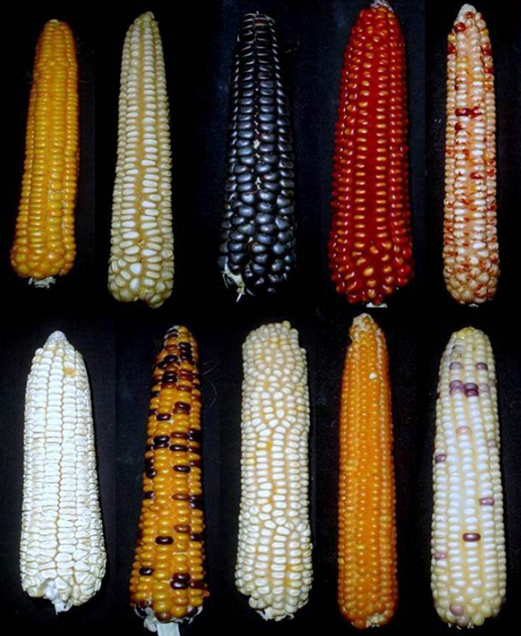
\includegraphics[width=\paperwidth,height=\paperheight]{MaizeLandrace2}
% }
\defbeamertemplate{background canvas}{mydefault}{}

\defbeamertemplate{background canvas}{standout}{%
  \centering
  \begin{tikzpicture}
  \node[opacity=0.2] {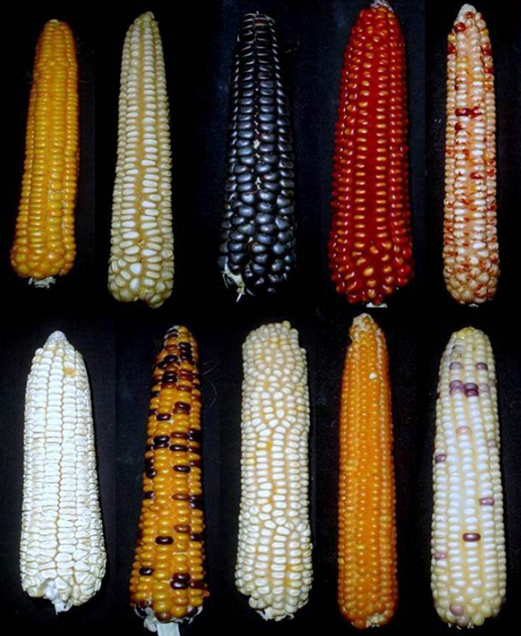
\includegraphics[height=\paperheight]{MaizeLandrace2}};
  \end{tikzpicture}
}

\BeforeBeginEnvironment{frame}{%
  \setbeamertemplate{background canvas}[mydefault]%
}

\makeatletter
\define@key{beamerframe}{standout}[true]{%
  \setbeamertemplate{background canvas}[standout]%
}
\makeatother